% !TeX root = ../main.tex
\chapter{Project 02: Target localization under sparse sensor attacks}

\section{Objectives}
The aim of this project is to localize the position of a device using RSS fingerprinting setting. In this project, we are given the dictionary $D$, and it is requested to localize the position of the device having a given measurement.

\section{Setting of the problem}
The localization problem is set in 10 by 10 squaremeters room. The room is gridded into 100 cells and 20 sensors are used in the training phase. In addition, it is assumed that during the training step has done in an offline manner, and therefore, the dictionary $D$ is assumed to be attack free. During the ``routine'' phase, which it is required to locate the position of the device, it is considered that 5 sensors are under attack, and the task is to localize the position of 1 target in this room given a vector of measurements. Therefore, the dimensions of the problem are as follows:
\begin{figure}[H] % h means "here", can also use t (top), b (bottom), p (page)
    \centering
    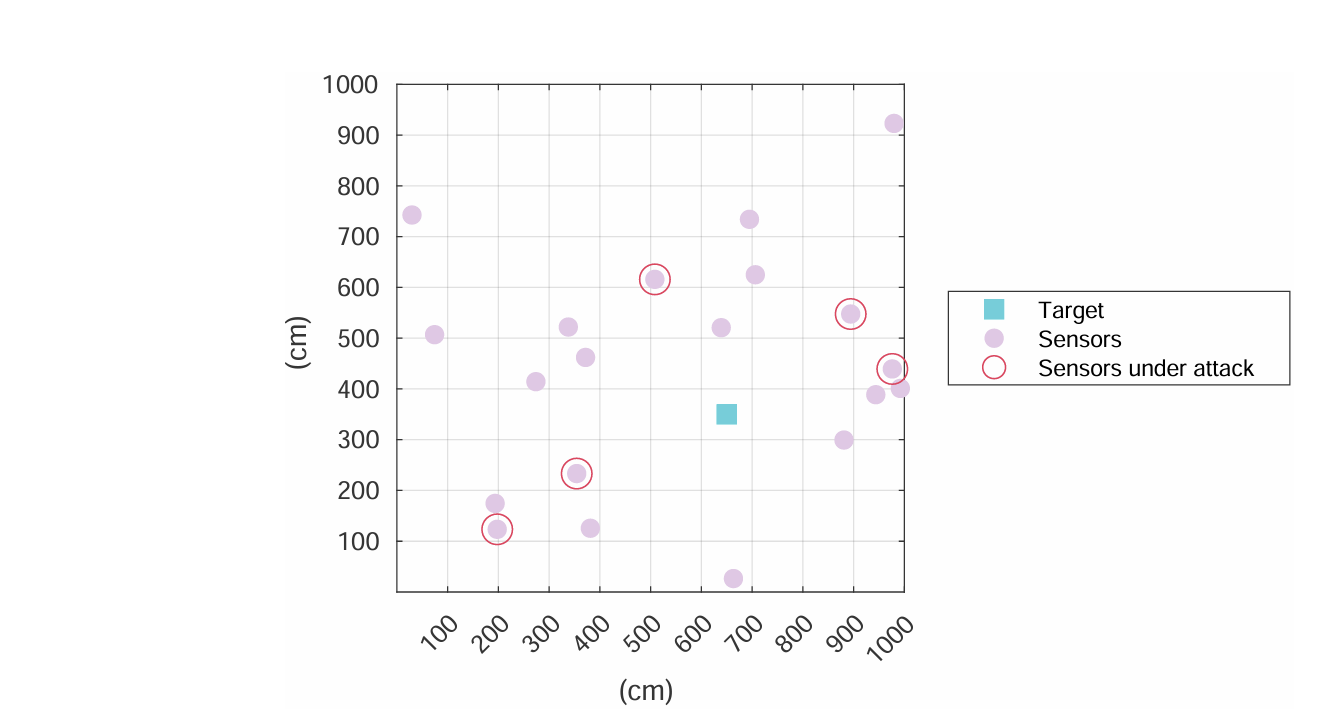
\includegraphics[width=0.75\textwidth]{localization_setting.png} % Adjust width as needed
    \caption{The graphical setting of the problem; reported from the project 2025 file.}
\end{figure}
\begin{itemize}
	\item the number of the cells (states) $n = 100$,  states can be 0 or 1, and only 1 state can be 1.
	\item the number of the sensors, length of the measurement sensor $q = 20$
	\item the number of the attacks $h = 5$
\end{itemize}

The same as the previous project, the problem to be solved is sparse. The diffence is that this time both the state vector and the attack vectors are expected to be sparse. Hence, a full weighted Lasso needs to be considered:

\begin{equation}
\min_{x \in \mathbb{R}^{n}, a \in \mathbb{R}^{q}} \left\| G \begin{pmatrix} x \\ a \end{pmatrix} - y \right\|_2^2 + \lambda_1 \| x \|_1 + \lambda_2 \| a \|_1
\end{equation}
where,
\[
G = (D, I)
\]

Here, in order not to face numerical problems, G should be normalized, this is done using \texttt{normalize( )} command in MATLAB. In this way, we make sure that $G$ and $I$ are of the same scale.

\section{Implementation of the algorithm}
The iterative algorithm used in order to converge to the solution of weighted Lasso is simular to the one implemented in the first project, with the difference that, since we know here also the state vector is going to be sparse, the soft-thresholding is used both for the attack and state vectors. Hence, after the initialization of the state and attack vectors, the following algorithm is implemented:

\begin{equation}
\begin{pmatrix}
x(k+1) \\
a(k+1)
\end{pmatrix}
=
\mathcal{S}_{\nu \lambda} \left[
\begin{pmatrix}
x(k) \\
a(k)
\end{pmatrix}
- \nu G^\top \left(
G \begin{pmatrix}
x(k) \\
a(k)
\end{pmatrix}
- y
\right)
\right]
\end{equation}

The suggested parameters for this problem is:
\begin{itemize}
	\item $\lambda_1 = \lambda_2 = 10$
	\item $\nu = \|G\|_2^2$
\end{itemize}

This algorithm is run until the difference of the two consequitive states becomes lower that $\delta = 10^{-10}$.

Once this goal is achieved, the state position needs to be cleaned. That is, 0 should be allocated to the states with values smaller than a certain threshold, and 1 should be allocated otherwise. In the given problem, it cannot be expected that, after performing cleaning, the state vector have more than one non-zero component - having only one target. At the end of  this step, both the position of the target and the position of the attacks are estimated, given the sensor measurements.

In order to estimate the correct values of attack, a support matrix corresponding the position of the attacks needs to be shaped. Then, the correct value of the attacks can be calculated as follows:

\begin{equation}
	\hat{a} = S_a^{+} \left( y - D \hat{x}_{cleaned}\right)
\end{equation}

In an attemp to enhance the performance of the algorithm the following values were used as hyperparameters:
\begin{itemize}
	\item $\nu = 0.0033$
	\item $\lambda_1 = 14$
	\item $\lambda_2 = 11.4$
\end{itemize}


\section{Results,}
Having run the algorithms for both suggested and enhance hyperparameters, the following table was obtained.

\begin{table}[ht]
\centering
\begin{tabular}{|c|c|c|c|}
\hline
\textbf{items} & \textbf{Real Data} & \textbf{suggested parameters} & \textbf{enhanced parameters} \\ \hline
\textbf{Iteration} & **** & 3752 & 1358 \\ \hline
\textbf{Attack Position} & \{1, 10, 14, 16, 17\} & \{1, 10, 14, 16, 17\} & \{1, 10, 14, 16, 17\} \\ \hline
\textbf{Target Position} & cell 37 & cell 37 & cell 37 \\ \hline
\end{tabular}
\caption{The results of running the algorithm with suggested and enhanced hyperparameters}
\end{table}

The estimated values of the attack are as follows:

\begin{figure}[H] % h means "here", can also use t (top), b (bottom), p (page)
    \centering
    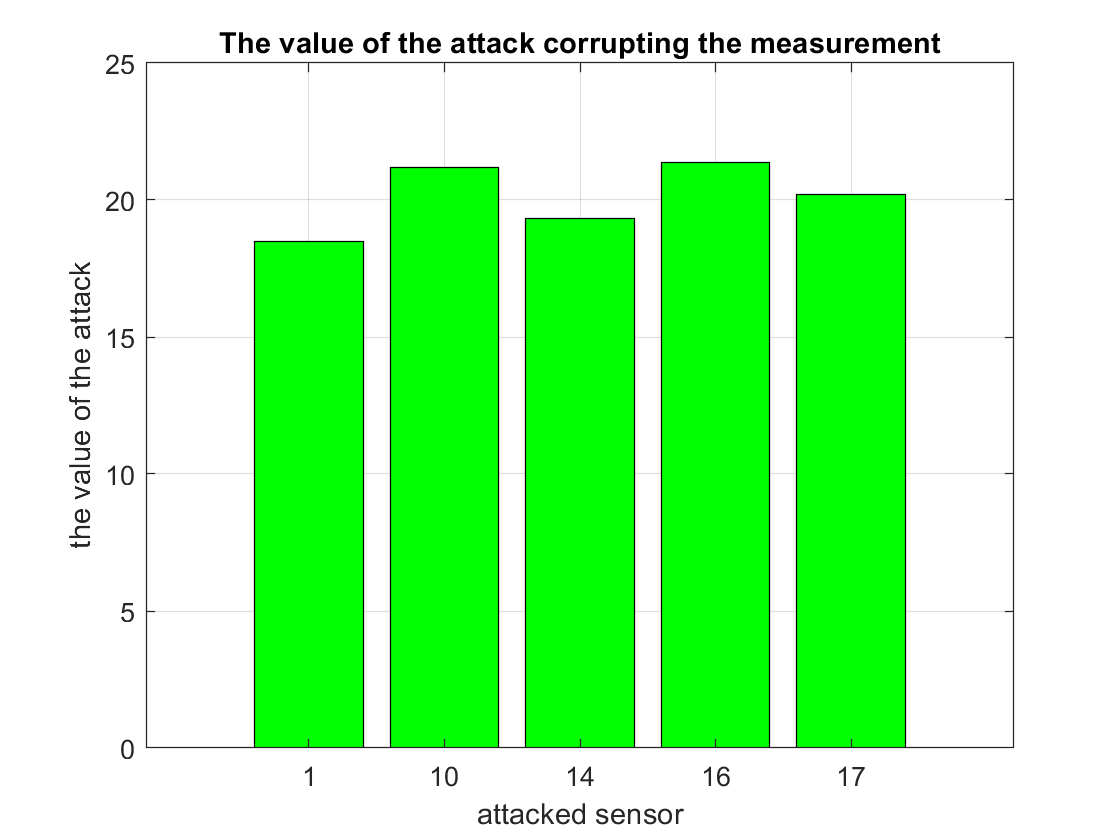
\includegraphics[width=0.5\textwidth]{attack_values.png} % Adjust width as needed
    \caption{The bar plot of the value of the attacks corrupting the sensors}
\end{figure}

\section{Further discussion: }
\subsection{why not IJAM?}
Regardless of the dimension of the problem, IJAM ``aggressive'' transient combined with soft-thresholding does not result in a good performance, since in the iterations where the value of the states drops suddenly, the soft-thresholding cuts those value. If the number of sensors are more than the number of cell the following steps can be followed:

\begin{enumerate}
	\item Having a transient phase where soft-thresholding is not applied to the state and we weight so that the transient passes. This can be coded by setting a threshold to check the difference in two consequetive state update is lower than a certain value.
	\item Then, we include soft-thresholding also for the state.
\end{enumerate}

However, in the problem at hand, the number of sensors are less than the number of cells and intrinsically underdetermined, and solving the problem with the psuedo inverse does not lead to an absolute minimum. 

\subsection{finding the position of the sensor}
Having the matrix $D$, the position of the sensors can be easily find. As each row of $D$ includes the signal strength of target in different cells, it is reasonable that the maximum element of each row, corresponds the cell that the signal is closer to, and therefore, the position of the sensor. The position of the sensors obtained are as follows:

\begin{table}[ht]
\centering
\caption{The number of the cell in which each sensor is places.}
\label{tab:sensor_positions}
\begin{tabular}{cc|cc}
\hline
\textbf{Sensor \#} & \textbf{Position} & \textbf{Sensor \#} & \textbf{Position} \\ \hline
1  & 66  & 11 & 54  \\
2  & 77  & 12 & 71  \\
3  & 43  & 13 & 44  \\
4  & 14  & 14 & 12  \\
5  & 7   & 15 & 50  \\
6  & 51  & 16 & 59  \\
7  & 29  & 17 & 24  \\
8  & 40  & 18 & 57  \\
9  & 68  & 19 & 12  \\
10 & 50  & 20 & 100 \\ \hline
\end{tabular}
\end{table}

The grafical representation of the sensors in the room can be compared to the actual setting in the following plot.

\begin{figure}[H]
    \centering
    \subfloat[The number of sensors in each cell]{
        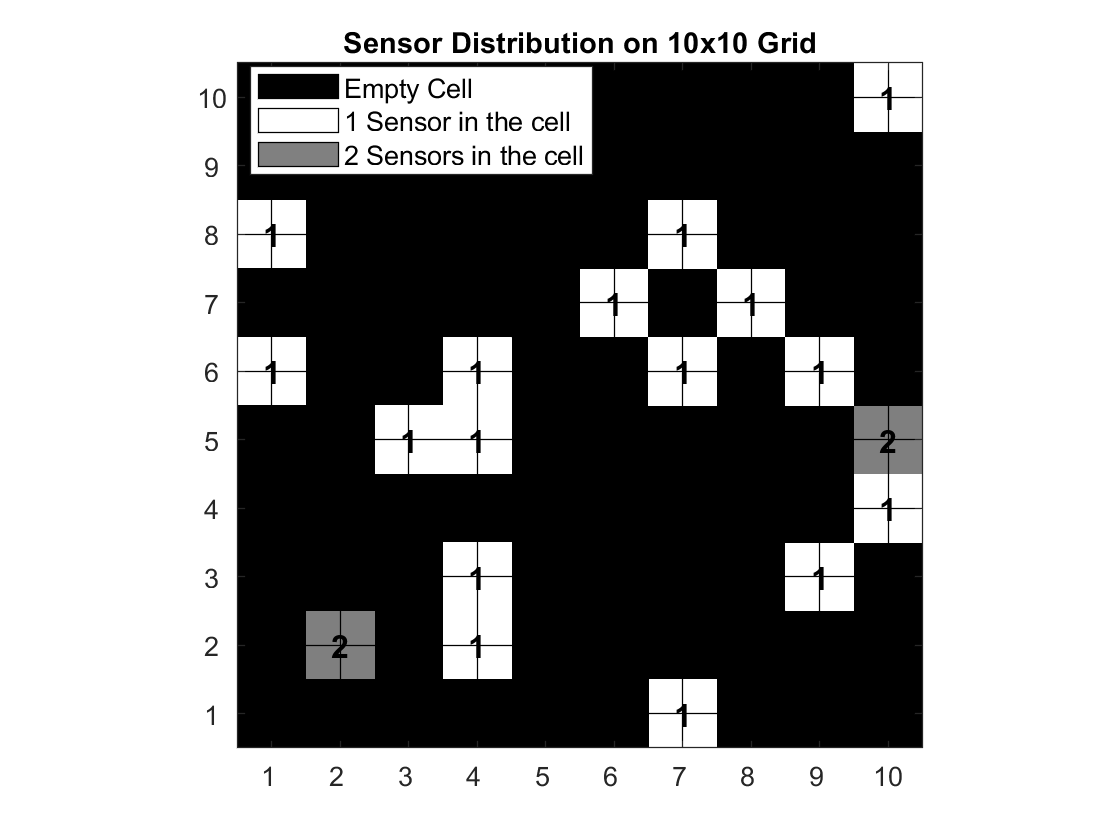
\includegraphics[width=0.35\textwidth]{sensor_position.png} % Adjust width as needed
    }
    \hspace{1cm} % Adjust the space between the two figures
    \subfloat[The head map of the attack support vector of different nodes after the consensus in the Star topology.]{
        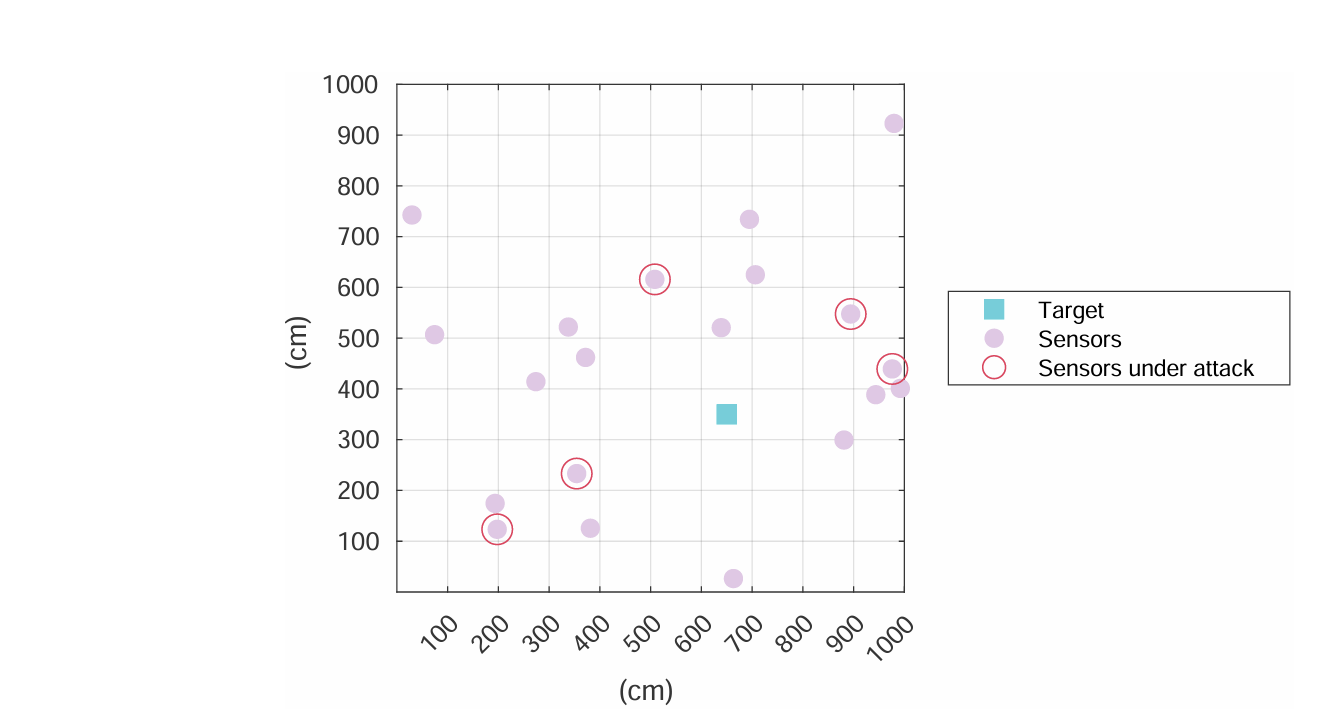
\includegraphics[width=0.55\textwidth]{localization_setting.png} % Adjust width as needed
    }
    \caption{The real and the estimated position of the sensors under attack.}
\end{figure}

\subsection{Localization using 1 attack-free sensors and not 3. How is it possible?}
From geometrical point of view, 3 sensors should be adopted in order to obtain a unique point in a plane. However, during the dictionary shaping, the center of the cells are used for placing the target, and the sensors are placed near the boarder of the cells. For this reason, considering any given cell and any given sensors, the arc that passes from the center of the cell does not passes the center of another cell, and thereby the measurement of target signal from the center of any cell would not be exactly the same as the measurements taken from the center of another cell, even if geometrically they both approximately have the same distance from the sensor. All in all, one attack-free, precise-enough sensor must be enough so as to locate the position of the target placed at the center of cells. In our case, using the sensor number 5, 6, 7, 11, 18, and 19 the position of the target was located in the following manner.

\texttt{[\~ \,, position] = min(D(sensorNumber,:) - y(sensorNumber))}

In our case, one cannot be sure whether the measurements are accurate enough to lead to the same result for measurement of other cell. Then, taking the effect of noises in to account, two sensors may be adopted for doing so.

\texttt{[\~ \,, position] = min(vecnorm(D([2, 3],:) - y(2:3),2,1))}

This was perfromed with some other 2 pairs of sensors, and the correct result was obtained each time. 


\section{Conclusion}
It can be seen that ISTA algorithm converges to the solution of weighted Lasso, and can correctly detect the position of the target as well as the position of the attacks sensors and the value of the attack. It was observed that the enhanced hyperparameter values led to a convergence rate that was twice as fast as the suggested values.

Since IJAM does not enjoy a smooth transient, the introduction of soft-thresholding disrupts converging to the solution of the problem. However, it is proposed a two step algorithm for implementing IJAM: 1) running normal IJAM so that the transient passes without applying soft-thresholding to the states, 2) applying soft-thresholding also to the states.

Having the matrix D, the position of sensors can be easily found, thanks to the fact that given a constant sensor, or at any rate row of the matrix D, the highest value correspond to the cell where that sensor is closer too, and hence the position of the sensor.

Further, it was observed that using 1 attack-free, precise sensor, the position of the target can be located in a plane. Nonetheless, to take in to considerations the effect of measurement noise, 2 sensor can be adopted for doing so, still the number of sensors adopted are lower than geometrical intuition suggest for localization in a plane.








